\documentclass[12pt, oneside,openright]{report} %Letter,
\usepackage[colorlinks=true, linkcolor=black, citecolor=blue, urlcolor = blue]{hyperref}
\usepackage[left=2.54cm, right=2.54cm, top=2.54cm, bottom=2.54cm]{geometry}
\usepackage[spanish]{babel}
\usepackage[table]{xcolor}
\usepackage{algpseudocode}
\usepackage[T1]{fontenc}
\usepackage{algorithm}
\usepackage{fancyhdr}
\usepackage{setspace}
\usepackage{pdfpages}
\usepackage{multirow}
\usepackage{listings}
\usepackage{graphics}
\usepackage{amsfonts}
\usepackage{graphicx}
\usepackage{amssymb}
\usepackage{amsmath}
\usepackage{amsthm}
\usepackage{epsfig}
\usepackage{subfig}
\usepackage{anyfontsize}
\usepackage{dirtytalk}
\usepackage{array}
\usepackage{tabularx}
\usepackage{textcomp}
\usepackage[utf8]{inputenc}
\usepackage[backend=biber,style=ieee, sorting=none, style=numeric]{biblatex}
\bibliography{Referencias}

    
\lstdefinestyle{mystyle}{
  keywordstyle=\color{blue},
  basicstyle=\ttfamily\footnotesize,
  breakatwhitespace=false,         
  breaklines=true,                 
  captionpos=b,                    
  keepspaces=true,                                 
  showspaces=false,                
  showstringspaces=false,
  showtabs=false,                  
  tabsize=1
}\lstset{style=mystyle}


\newtheorem{definition}{Definición}
\newtheorem{theorem}{Teorema}

\renewcommand{\lstlistingname}{Codigo}

\renewcommand{\algorithmicrequire}{\textbf{Input:}}
\renewcommand{\algorithmicensure}{\textbf{Output:}}
\renewcommand{\lstlistlistingname}{Índice de Códigos}

\newenvironment{resumen}
  {\cleardoublepage\thispagestyle{plain}\vspace*{\stretch{1}}\begin{center}\bfseries Resumen.\end{center}}
  {\vspace*{\stretch{2}}}

\newenvironment{_abstract1}
  {\cleardoublepage\thispagestyle{plain}\vspace*{\stretch{1}}\begin{center}\bfseries Abstract1\end{center}}
  {\vspace*{\stretch{2}}}
% \makeatletter

% \makeatother

\begin{document}

\makeatletter
  \renewcommand{\ALG@name}{Algoritmo}
\makeatother
  
\renewcommand{\listtablename}{Índice de tablas}
\renewcommand{\tablename}{Tabla}

\begin{titlepage}
\begin{minipage}[l]{3.5cm}

\includegraphics[width=5cm, height=22.0cm]{imagenes/Imagen_front_UPTex.jpg}
\end{minipage}
\vspace*{-3.0cm}
\begin{minipage}[r]{13.0cm}
\begin{center}
\textbf{\LARGE{UNIVERSIDAD POLIT\'{E}CNICA }}\\
\vspace*{0.5cm}
\textbf{\LARGE{DE TEXCOCO}} \\
\vspace*{2.0cm}
\large{\textbf{NOMBRE DE LA MEMORIA} \\

\vspace*{0.5cm}

\vspace*{0.5cm}

\vspace*{1.0cm}
\textbf{P R E S E N T A:} \\
\vspace*{0.5cm}
\textbf{AUTOR(es):} \\

\textbf{}\\
\vspace*{1.0cm}

\vspace*{0.5cm}

\vspace*{1.5cm}
TEXCOCO, EDO. MÉX. \hspace{3cm}ENERO 2025 \\
\end{center}
\end{minipage}
\end{titlepage}
\spacing{1.5}   
\pagenumbering{Roman} \setcounter{page}{2}

\newpage
\section*{Resumen.}

En este estudio, se introduce una modificación a la técnica tradicional del controlador de saturación anidado (NSC) utilizada para la estabilización de vehículos aéreos con despegue y aterrizaje vertical (PVTOL-UAV). La propuesta consiste en incorporar funciones hiperbólicas suaves dentro de la configuración anidada del NSC, con el objetivo de desarrollar un algoritmo de control avanzado que optimice tanto el tiempo de convergencia como el rendimiento en lazo cerrado del sistema. 

El enfoque planteado utiliza el error en los estados del sistema como señal de realimentación, permitiendo que la pendiente de la función hiperbólica acotada sea ajustable, lo que facilita la sintonización precisa de la respuesta del controlador. Esta capacidad de ajuste permite una rápida convergencia de los estados hacia los valores deseados, mejorando la estabilidad y la eficiencia del sistema controlado.

Los resultados del estudio se obtienen mediante simulaciones numéricas, donde se realiza una comparación gráfica entre el desempeño del controlador propuesto y el controlador NSC clásico, ambos aplicados al modelo dinámico del PVTOL. Además, se implementa una variante del control anidado difuso sobre el mismo modelo matemático para comparar su desempeño con el del nuevo controlador propuesto, utilizando un valor del parámetro $K = 0.05$. Las simulaciones demuestran que el controlador basado en funciones hiperbólicas suaves, con saturaciones anidadas, logra un tiempo de convergencia significativamente mejorado en comparación con las alternativas tradicionales.

\addcontentsline{toc}{chapter}{Resumen}
\newpage
\section*{Abstract.}

In this study, a modification to the traditional nested saturation controller (NSC) technique used for vertical take-off and landing aerial vehicle (PVTOL-UAV) stabilization is introduced. The proposal consists of incorporating smooth hyperbolic functions within the nested NSC configuration, with the objective of developing an advanced control algorithm that optimizes both the convergence time and the closed-loop performance of the system.
The proposed approach uses the error in the system states as a feedback signal, allowing the slope of the bounded hyperbolic function to be adjustable, which facilitates accurate tuning of the controller response. This fine-tuning of the controller response is facilitated by this tunability. This tunability allows rapid convergence of the states to the desired values, improving the stability and efficiency of the controlled system
The results of the study are obtained through numerical simulations, where a graphical comparison is made between the performance of the proposed controller and the classical NSC controller, both applied to the dynamic model of the PVTOL. In addition, a variant of the nested fuzzy control is implemented on the same mathematical model to compare its performance with that of the new proposed controller, using a value of the parameter K = 0.05. The simulations show that the controller based on smooth hyperbolic functions, with nested saturations, achieves a significantly improved convergence time compared to traditional alternatives.

\addcontentsline{toc}{chapter}{Abstract}
\newpage 


%\begin{spacing}{1.5}
    \tableofcontents
    \newpage
    \listoffigures
    \newpage
    \listoftables    
    \newpage
    %\input{acronimos.tex}
%\end{spacing}


\pagenumbering{arabic} \setcounter{page}{1} % Números arábigos para el contenido principal


\chapter{Marco de Referencia}

 Desde finales del siglo pasado, los avances tecnológicos en la miniaturización de la electrónica y los componentes mecánicos han allanado el camino para la creación y desarrollo de objetos voladores de pequeñas dimensiones, tales como aviones y helicópteros, los cuales están adquiriendo cada vez más habilidades para realizar vuelos de forma autónoma. Estos dispositivos son popularmente conocidos como drones, un término derivado del inglés \say{abejorros}, y se consideran máquinas voladoras autónomas o semi-autónomas capaces de llevar a cabo misiones de vuelo. En el ámbito internacional, se les conoce como UAVs del ingles \say{Unmanned Aerial Vehicles}, y representan una tecnología compleja cuyo control presenta desafíos, dado que sus características aerodinámicas son similares a las de las aeronaves convencionales \cite{eisenbeiss2004mini}.

El estudio de estos dispositivos despierta un gran interés debido a su versatilidad y capacidad de maniobra, lo que les permite llevar a cabo una amplia gama de tareas en diversas aplicaciones, tales como el uso civil, militar y aeroespacial \cite{nawaz2019applications, shakhatreh2019unmanned, xiaoning2020analysis}. En la figura \ref{fig1_aplicacion_UAV}, se presenta una clasificación detallada de las aplicaciones más importantes de los UAVs.

\begin{figure}[H]
    \centering
    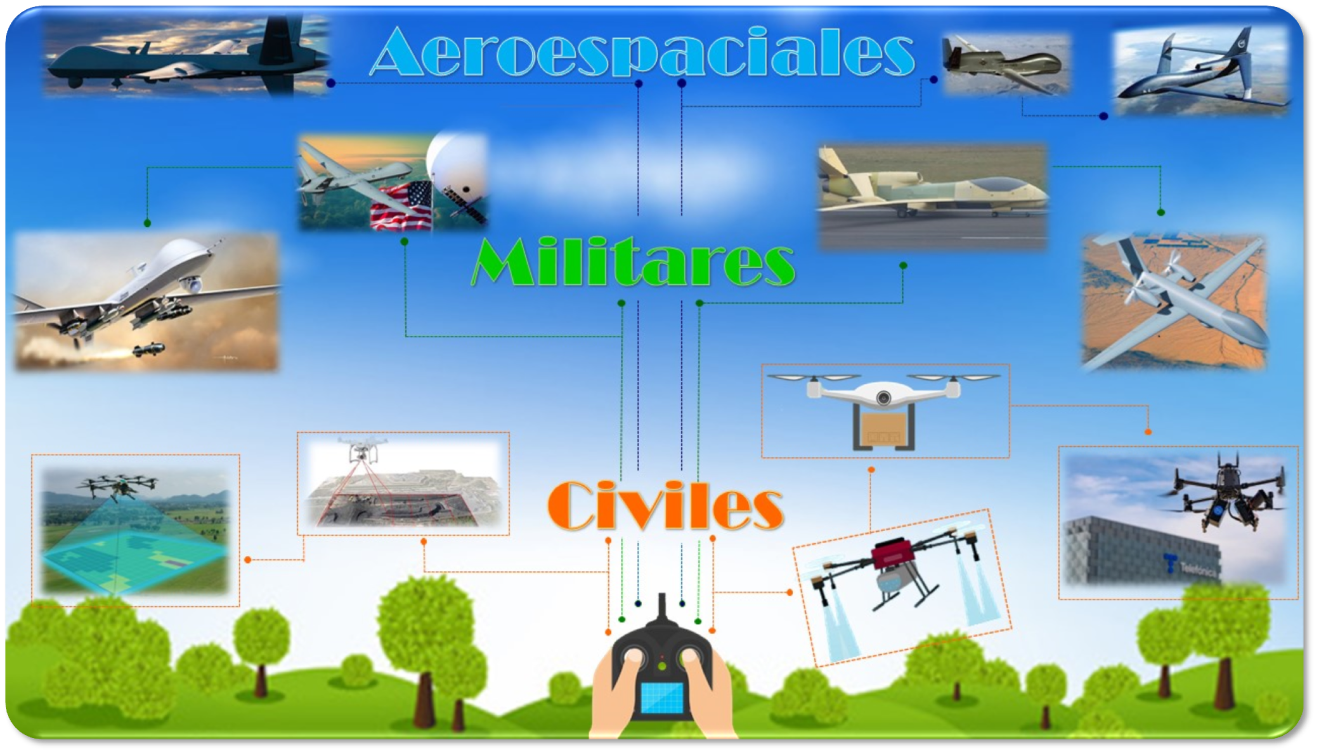
\includegraphics[width=16cm, height=7.5cm]{imagenes/Aplicaciones_UAV.png}
    \caption{Áreas de aplicación UAVS.}
    \label{fig1_aplicacion_UAV}
\end{figure}

\section{Antecedentes.}

Los drones han atraído la atención de la comunidad investigadora que trabaja tanto en el campo militar como en el civil, con una gran cantidad de usos que han sido propuestos por los grupos de investigación, debido a sus características como capacidad y configuraciones, donde el helicóptero de cuatro rotores tiene el mayor número de citas en la literatura de control y ha sido ampliamente investigado para pruebas tanto en interiores como en exteriores . 

\section{Objetivo General}
\textbf{}
\section{Objetivos Especificos}
\begin{enumerate}
\item Recolectar y organizar conjuntos de datos públicos internacionales sobre calidad del aire, variables meteorológicas y factores geoespaciales. 
\item Explorar y analizar las principales tendencias, correlaciones y patrones de comportamiento entre los contaminantes atmosféricos y las variables ambientales, utilizando técnicas de análisis exploratorio de datos.

\end{enumerate}

\section{Alcance}
El proyecto comprenderá el diseño, desarrollo y validación de una aplicación web para la gestión de recursos materiales y de incidencias de mantenimiento e infraestructura en un plantel universitario. Su organización seguirá la arquitectura Modelo–Vista–Controlador (MVC), con Laravel y una base de datos MariaDB. El acceso se realizará mediante cuentas de correo institucional y permisos diferenciados para solicitantes, coordinación, personal técnico y personal de almacén; la administración de usuarios y roles quedará reservada al personal autorizado.
El sistema contemplará el registro de fallas asociadas a edificios y espacios del plantel, con descripción y evidencia fotográfica; la consulta y el seguimiento de los reportes; y su revisión por parte de coordinación. Se incluirán mecanismos para prevenir reportes repetidos y agrupar aquellos que correspondan a una misma incidencia, así como la asignación de técnicos considerando especialidad y turno y la autorización de trabajos que lo requieran por su costo o riesgo.
La gestión operativa abarcará las órdenes de trabajo, el registro de tareas y estados de atención, la solicitud y entrega de materiales, las entradas y salidas de inventario y la consulta de existencias. Las operaciones relevantes se registrarán en bitácora para relacionar reportes, responsables, movimientos de materiales y evidencias de cierre. El cierre de una orden contemplará la comprobación de tareas y el registro de evidencia del trabajo realizado.
La entrega incluirá la documentación técnica y de uso, el modelo de base de datos y las pruebas funcionales, de seguridad y de flujo por rol necesarias para demostrar el proceso de atención de una incidencia. Las funciones descritas constituyen el alcance previsto del proyecto y su cumplimiento se verificará durante las pruebas.


\section{Limitación}
\begin{enumerate}
\item \textbf{Cobertura institucional.} La primera versión se delimitará a un plantel universitario y a los edificios, espacios, usuarios y materiales incorporados a sus catálogos. No se contempla la administración centralizada de múltiples instituciones.

\item \textbf{Entorno de operación.} El uso del sistema dependerá de la disponibilidad de un servidor con PHP y Laravel, una base de datos MariaDB, almacenamiento para las evidencias y acceso a la red desde un navegador compatible. No se contempla una aplicación móvil nativa ni el registro y la sincronización de operaciones sin conexión.

\item \textbf{Dependencia de los datos y de la operación humana.} La calidad del seguimiento dependerá de la captura correcta y oportuna de reportes, asignaciones, movimientos y evidencias por parte de los usuarios autorizados. La identificación de posibles duplicados requerirá revisión de coordinación; el sistema no garantizará la detección automática de todas las incidencias repetidas.

\item \textbf{Integraciones y procesos externos.} No se incluyen integraciones con sistemas institucionales externos, compras, pagos, contabilidad, dispositivos biométricos ni firma electrónica certificada. El control de almacén se enfocará en existencias y movimientos vinculados con la atención de incidencias; no abarcará la gestión completa del ciclo de vida de los activos.

\item \textbf{Validación y tiempos de atención.} Las pruebas se efectuarán con los recursos y escenarios disponibles durante el desarrollo académico. Los resultados de rendimiento se limitarán al entorno y a la carga evaluados. La aplicación apoyará la coordinación y el seguimiento, pero no garantizará un plazo fijo de reparación, ya que este dependerá de la disponibilidad de personal, materiales y autorizaciones.
\end{enumerate}


\section{Problemática}


\section{Justificación}


\chapter{Marco Teórico.}

En el desarrollo de sistemas de control para vehículos aéreos no tripulados (UAVs), los Vehículos de Despegue y Aterrizaje Vertical (VTOL, por sus siglas en inglés) y sus variantes Planas (PVTOL) han captado una atención significativa debido a sus aplicaciones en diversas áreas como la vigilancia \cite{johnson1997arti}, entrega de paquetes \cite{9129495} y exploración \cite{5278262}. Este capítulo aborda los principios teóricos que respaldan el diseño y control de estos vehículos, incluyendo modelos matemáticos y técnicas avanzadas de control.
En primer lugar, se describen los enfoques de modelado matemático utilizados para representar el comportamiento dinámico de los VTOL y PVTOL. Estos modelos son esenciales para comprender y predecir las respuestas del sistema ante diferentes estímulos. Particularmente, se emplea el formalismo de Euler-Lagrange, un método robusto y ampliamente aceptado en la dinámica de sistemas mecánicos.

\section{Sección}

La capacidad de despegue y aterrizaje vertical (VTOL) es muy apreciada en los vehículos aéreos no tripulados (UAV) y tripulados (MAV), siempre que se alcance un rendimiento de vuelo comparable. La tecnología VTOL no solo resulta muy adecuada para los UAV debido a los requisitos de misión y la necesidad de ocultación, sino que también es de gran importancia para los MAV, tanto en aplicaciones militares como civiles, debido a las ventajas que ofrece, como una menor o incluso nula dependencia de aeropuertos o campos de aviación.

\section{Sección 2}

El modelo PVTOL (Plataforma Vertical Despegue y Aterrizaje) describe el movimiento vertical de un objeto en un plano, caracterizado por tres grados de libertad $(x, y, \phi)$ que corresponden a la posición y la orientación del objeto en dicho plano. Este sistema incluye dos propulsores independientes que generan fuerzas y momentos en la máquina voladora, como se muestra en la figura \ref{fig1:PVTOL}. Es importante destacar que el PVTOL es un sistema subactuado, ya que aunque tiene tres grados de libertad, solo cuenta con dos entradas para su control. Debido a esta característica, el PVTOL constituye un desafío significativo en el ámbito del control no lineal \cite{lin1999robust}.


\subsection{Subsección}
El modelado y diseño de control para plataformas UAV es un trabajo difícil debido a su complicada estructura no lineal y subactuada, donde su comportamiento es función de efectos aerodinámicos, estructura mecánica, perturbaciones, incertidumbre, etc. 

\section{Modelos matemáticos.}

Para entender los sistemas, es esencial desarrollar modelos matemáticos que los representen con exactitud. Un modelo de un sistema se describe como una representación de sus características relevantes, y el proceso de abstracción necesario para crear esta representación se conoce como modelado. El modelo es una versión simplificada de una realidad compleja; el término \say{modelar}se refiere a crear una descripción que capture de manera precisa un sistema y sus actividades. Los modelos científicos se desarrollan para realizar inferencias sobre ciertos aspectos de sistemas reales previamente observados. Este proceso de creación y utilización de un modelo se ilustra en la figura \ref{fig: tipos de modelo} a). Estos modelos se pueden clasificar de acuerdo al conocimiento previo sobre el proceso ilustrados en la figura \ref{fig: tipos de modelo} b).

\begin{figure}[H]
    \centering
    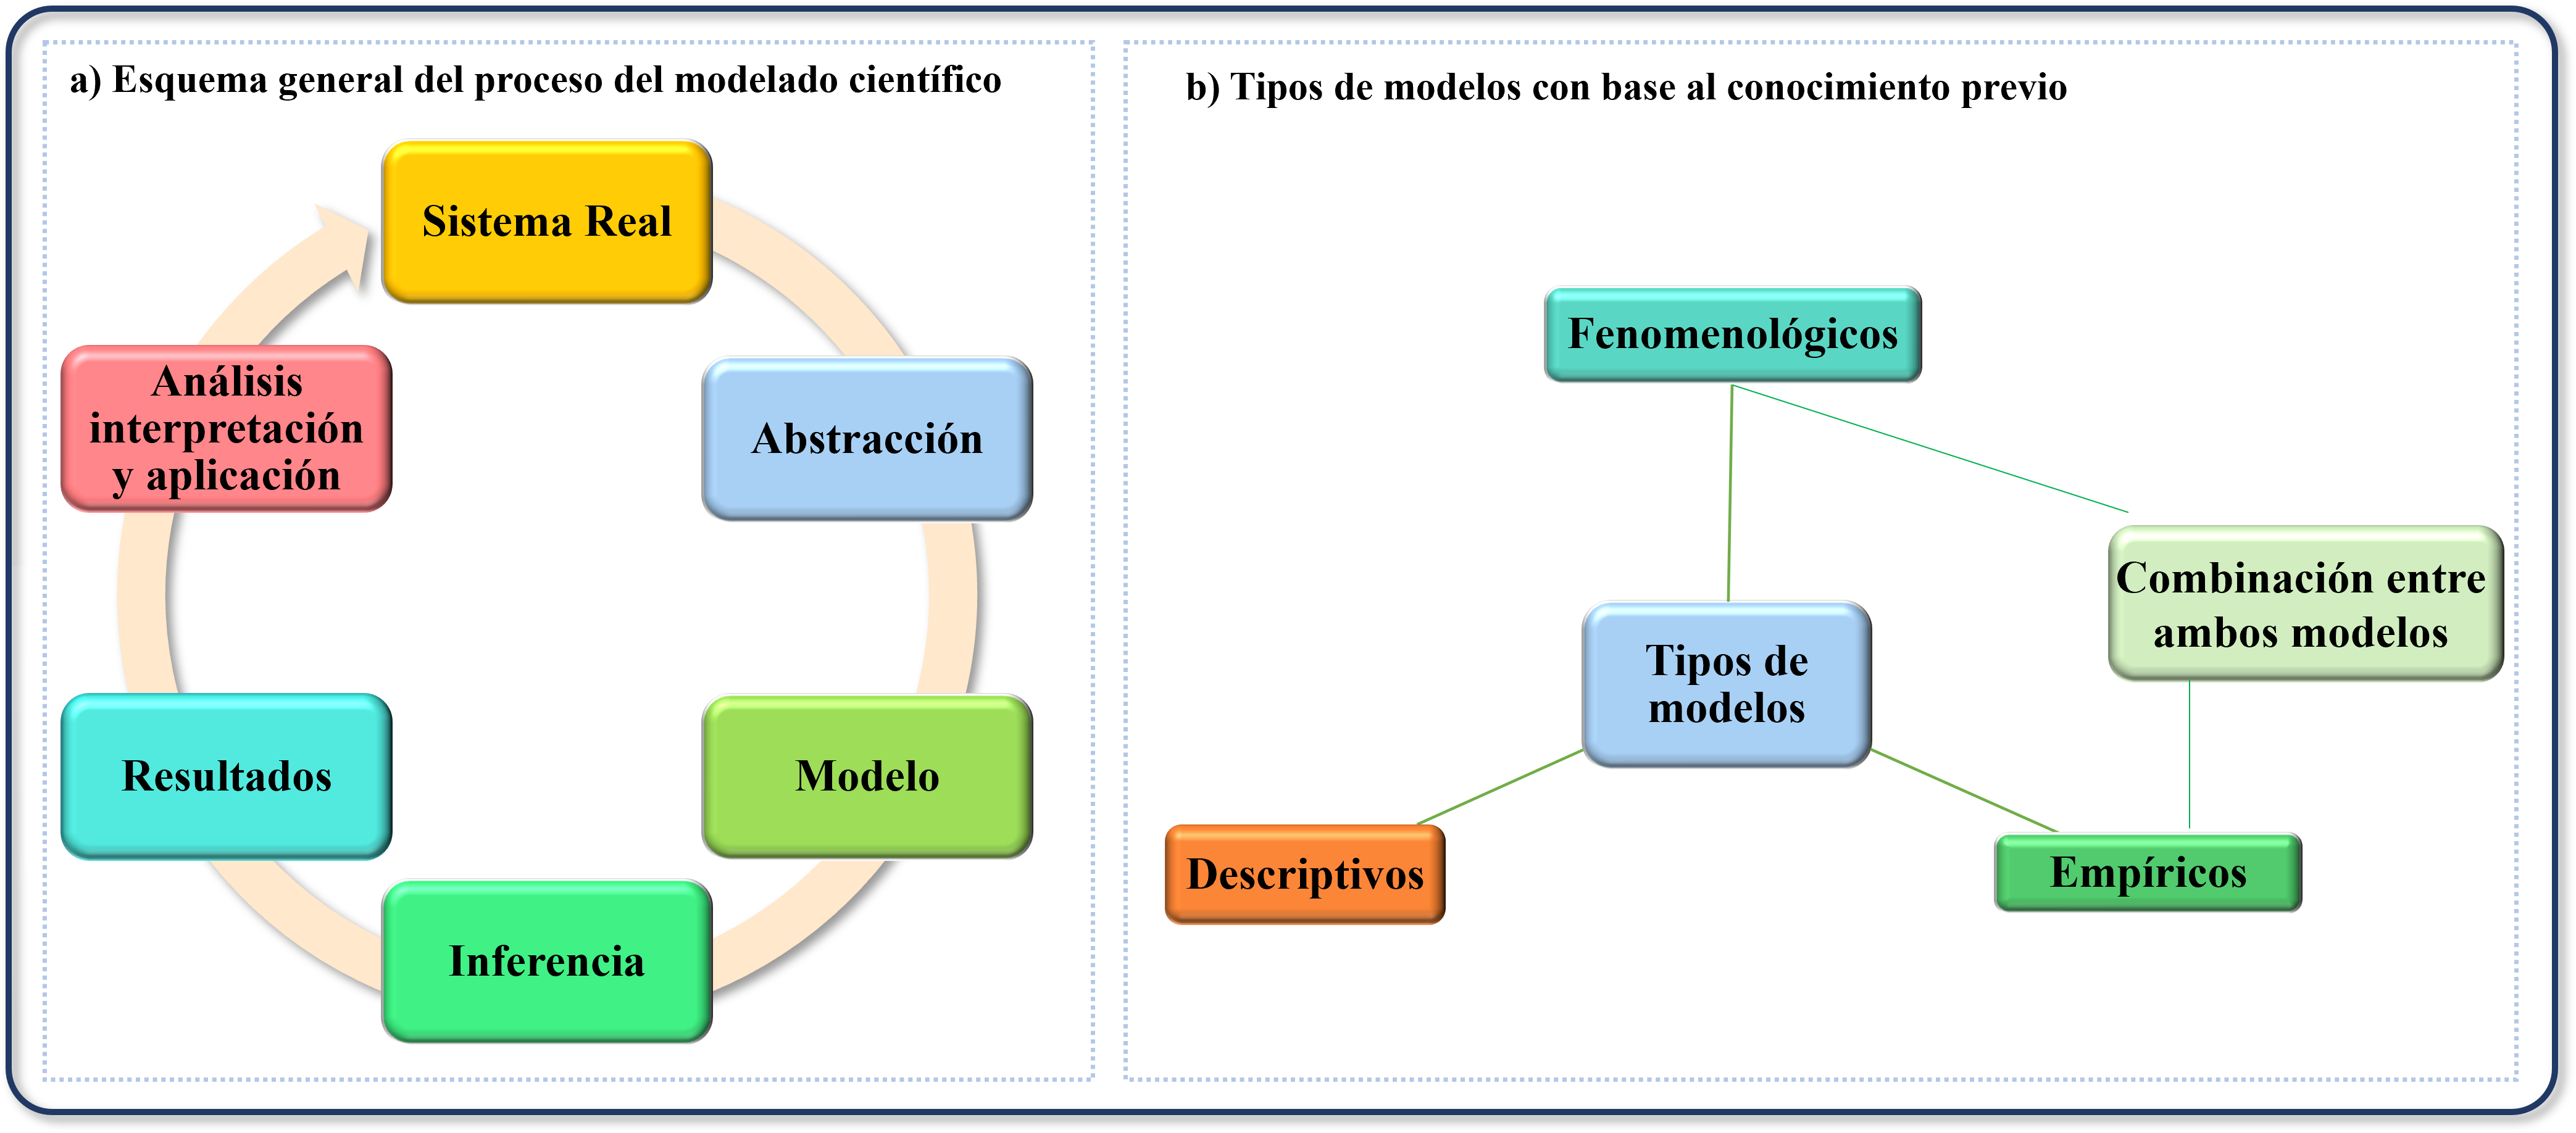
\includegraphics[width=\textwidth, height=8cm]{imagenes/esquema_modelado.png}
    \caption{Sistema de modelado.}
    \label{fig: tipos de modelo}
\end{figure}

Otra forma de modelar un sistema es mediante modelos matemáticos, los cuales replican las relaciones de entrada(s) - salida(s) utilizando expresiones matemáticas. Cuando existe una relación lineal entre la entrada y la salida, el modelo matemático se expresa como:
\begin{equation}
     y(t) = u(t)k_{p}
     \label{eq_modelo}
\end{equation}

Donde $y(t)$ es la salida, $u(t)$ es la entrada del sistema, y $k_{p}$ es la constante de proporcionalidad. No obstante, la ecuación (\ref{eq_modelo}) implica que cualquier cambio en la entrada se reflejará instantáneamente en la salida, lo cual no es cierto en sistemas reales, ya que la salida requiere tiempo para ajustarse. Esta relación se cumple únicamente cuando se ha alcanzado un tiempo suficiente para estabilizarse, conocido como la condición de estado estable, y puede representarse como:\\
\textit{El Valor en estado estable de $u(t)$ = $y(t)$ por el Valor en estado estable de $k_{p}$}
\begin{equation}
    k_{p} = \frac{y(t)}{u(t)}
\end{equation}

Donde $k_{p}$ se refiere a la ganancia del sistema o función de transferencia. Así, una función de transferencia se define como la relación entre la salida en estado estable y la entrada en estado estable de un sistema.

 
\subsection{Formalismo de Euler-Lagrange.}

La formulación Lagrangiana proporciona una forma de modelar la dinámica de un robot al analizar el balance de energía. En este enfoque, el robot se conceptualiza como una entidad cerrada, y las ecuaciones derivadas se centran únicamente en la energía almacenada, representada a través de las energías cinética y potencial. Para un robot dado, los resultados obtenidos mediante esta formulación son idénticos a los obtenidos mediante la formulación de Newton-Euler.
El Lagrangiano es una función escalar definida como la diferencia entre las energías cinética y potencial de un sistema mecánico, en función de las llamadas coordenadas generalizadas \cite{torres2002robots}. En la figura \ref{fig 2_2: Esquema de Euler_lagrange} se desarrolla en detalle la formulación Lagrangiana.


\begin{equation}
J_{i}=
    \begin{bmatrix}
        \lambda_{i} & 1           & 0      &...  & 0  \\
        0           & \lambda_{i} & 1      & ...& 0 \\
        \vdots      & \vdots      & \ddots & \ddots & \vdots \\
             0   &    0    &  ... & \lambda_{i} & 1   \\
           0 &   0   &  ...       &  0   & \lambda_{i} \\
    \end{bmatrix}_{m \times m}
\end{equation}

Donde $J_{i}$ es el bloque de Jordan asociado al eigenvalor $\lambda_{i}$  en $A$ y $m$ es el orden del bloque de Jordan. Esta representación es útil porque simplifica el análisis de la dinámica de sistemas lineales, especialmente cuando $A$ no es diagonalizable. La solución del sistema en términos de la forma de Jordan es:

\begin{equation}
     exp(at) = P exp(Jt) P^{-1} = \sum_{i=1}^{r}\sum_{k=1}^{m_{i}}t^{k-1}exp(\lambda_{i}t)R_{ik}
\end{equation}

Donde $m_{i}$ es el orden del bloque de  Jordan asociado al eigenvalor $A$. El siguiente teorema caracteriza las propiedades de estabilidad del origen.

\chapter{Desarrollo}
Desarrollo del proyecto, identifica la metodología  Agiles (sea SCRUM, KABAN, etc. )describe cada una de las fases del proceso de desarrollo de su proyecto. 
\chapter{Resultados}
Resultados



%\bibliographystyle{IEEEtran}
%\addcontentsline{toc}{chapter}{Referencias}

\printbibliography[title = {Referencias}]

\end{document}

